% F089｜勾股整数数组的构造规律｜02_explanation.tex
% 继承上传模板的 LaTeX 环境；当前条目的内容独立编写。
\clearpage
\begin{explanationbox}
\textbf{\textcolor{CExplanation}{为什么一定能构成直角三角形}}
\par\medskip
\begin{center}
% F089｜triangle 原创简明教学示意图
\begin{tikzpicture}[>=stealth,scale=.9]
\coordinate (A) at (0,0);\coordinate (B) at (4,0);\coordinate (C) at (0,3);
\fill[teal!12] (A)--(B)--(C)--cycle;\draw[very thick,teal] (A)--(B)--(C)--cycle;
\draw (.3,0)--(.3,.3)--(0,.3);
\node[below] at (2,0){$4$};\node[left] at (0,1.5){$3$};\node[right] at (2,1.6){$5$};
\node[anchor=west] at (5,2.1){$3^2+4^2=5^2$};
\node[anchor=west] at (5,1.3){\small 直角边的平方和};
\node[anchor=west] at (5,.8){\small 等于斜边平方};
\end{tikzpicture}

\end{center}
\medskip
把斜边平方展开：$(m^2+n^2)^2=m^4+2m^2n^2+n^4$。两直角边平方之和是 $(m^2-n^2)^2+(2mn)^2=m^4+2m^2n^2+n^4$，正好相等。
\end{explanationbox}
\clearpage
\begin{explanationbox}
\textbf{\textcolor{CExplanation}{奇数平方拆成两个相邻数}}
\par\medskip
\begin{center}
% F089｜odd 原创简明教学示意图
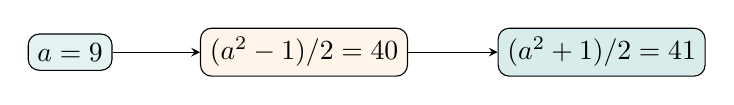
\begin{tikzpicture}[>=stealth,scale=.9]
\node[draw,fill=teal!10,rounded corners] (a) at (0,0){$a=9$};
\node[draw,fill=orange!8,rounded corners] (b) at (3.3,0){$(a^2-1)/2=40$};
\node[draw,fill=teal!15,rounded corners] (c) at (7.5,0){$(a^2+1)/2=41$};
\draw[->] (a)--(b);\draw[->] (b)--(c);
\end{tikzpicture}

\end{center}
\medskip
若直角边 $a$ 为大于1的奇数，则 $a^2$ 为奇数。令另两边为 $b$ 和 $b+1$，由 $a^2+(b)^2=(b+1)^2$，可得 $a^2=2b+1$，所以 $b=(a^2-1)/2$。例如 $a=9$ 得 $(9,40,41)$。
\end{explanationbox}
\clearpage
\begin{explanationbox}
\textbf{\textcolor{CExplanation}{偶数半数平方加减1}}
\par\medskip
\begin{center}
% F089｜even 原创简明教学示意图
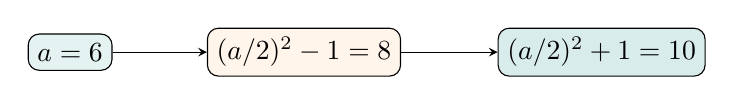
\begin{tikzpicture}[>=stealth,scale=.9]
\node[draw,fill=teal!10,rounded corners] (a) at (0,0){$a=6$};
\node[draw,fill=orange!8,rounded corners] (b) at (3.3,0){$(a/2)^2-1=8$};
\node[draw,fill=teal!15,rounded corners] (c) at (7.5,0){$(a/2)^2+1=10$};
\draw[->] (a)--(b);\draw[->] (b)--(c);
\end{tikzpicture}

\end{center}
\medskip
若 $a=2n$ 且 $n\ge2$，则 $(n^2+1)^2-(n^2-1)^2=4n^2=a^2$。例如 $a=8$，$n=4$，得到 $(8,15,17)$。
\end{explanationbox}
